% For tips on writing the thesis, see http://www.tug.org/pracjourn/2008-1/mori/mori.pdf

% Two side to save paper
% openrigth means to put the chapter tittle on the right pages
\documentclass[12pt,letterpaper,twoside,openright]{book}
\usepackage[utf8]{inputenc}
\usepackage[T1]{fontenc}
% Language support
\usepackage[english,spanish]{babel}

\usepackage[table,xcdraw]{xcolor}


\newenvironment{dedication}
{
   \cleardoublepage
   \thispagestyle{empty}
   \vspace*{\stretch{1}}
   \hfill\begin{minipage}[t]{0.66\textwidth}
   \raggedright
}%
{
   \end{minipage}
   \vspace*{\stretch{3}}
   \clearpage
}

\newenvironment{acreditation}
{
   \cleardoublepage
   \thispagestyle{empty}
   %\vspace*{\stretch{1}}
   
   %\raggedright
}%
{
   
   %\vspace*{\stretch{3}}
   \clearpage
} 


\newenvironment{notetoeditor}
{
   \begin{tcolorbox}[title={Nota al editor},colback=yellow!5!white]
}%
{
   \end{tcolorbox}
}

\newcommand*{\captionsource}[2]{%
	\caption[{#1}]{%
		#1%
		\\\hspace{\linewidth}%
		\textbf{Source:} #2%
	}%
}

\setcounter{tocdepth}{4}
\setcounter{secnumdepth}{4}

\selectlanguage{english}
%\usepackage[spanish]{datetime}

% We define some strings that will use along
\def \thesiskeywords {thesis, master degree, your topics here}
\def \pdfauthor {Erick Alejandro Muñoz Alvarado}
\def \thesistitle{TODO FIX: Uncertainty quantification for Whisper }

% Custom-commands and definitions
% See this file for defining the keywords that will show up on the PDF file
\input{../packages}

% =====================================================================
%  CUSTOMIZATION ZONE
%  Anything below \input{../packages} can safely use packages the
%  preamble loads (hyperref, xcolor, glossaries, ...). Put your own
%  \usepackage lines, \renewcommand's and custom macros HERE -- not
%  above \input{../packages}, or they may reference things not yet loaded.
% =====================================================================

% URL / link footnote styling
\renewcommand\UrlFont{\color{blue}\rmfamily}
\urlstyle{rm}

% EPS figures: convert on the fly with epstopdf. Writes the *-eps-converted-to.pdf
% files into build/ instead of next to the sources. Requires building with
% -shell-escape (see the build command in the repo notes).
\usepackage{epstopdf}
\epstopdfsetup{outdir=build/}

% ========================== RESULT VALUES ==========================
% Temperature Scaling
\newcommand{\tsTemp}{1.126}             % optimal temperature
\newcommand{\tsCalibrationR}{0.539}     % mean R on calibration dataset
\newcommand{\tsTestR}{0.439}            % mean R on test dataset
% Monte Carlo Dropout
\newcommand{\mcdRate}{0.003}            % optimal dropout rate
\newcommand{\mcdCalibrationR}{0.464}    % mean R on calibration dataset
\newcommand{\mcdTestR}{0.469}           % mean R on test dataset
% Levenshtein Monte Carlo Dropout
\newcommand{\lmcdRate}{0.037}           % optimal dropout rate
\newcommand{\lmcdCalibrationR}{0.716}   % mean R on calibration dataset
\newcommand{\lmcdTestR}{0.679}          % mean R on test dataset

% Layout toggle: 'true' = paper, 'false' = thesis (consumed in packages.tex)
\newtoggle{paper}
\settoggle{paper}{true}

% Acronyms
\makenoidxglossaries

\newacronym{ue}{UE}{Uncertainty Estimation}
\newacronym{uq}{UQ}{Uncertainty Quantification}
\newacronym{cmaes}{CMA-ES}{Covariance Matrix Adaptation Evolution Strategy}
\newacronym{mcd}{MCD}{Monte-Carlo Dropout}
\newacronym{lmcd}{LMCD}{Levenshtein Monte-Carlo Dropout}
\newacronym{ts}{TS}{Temperature Scaling}
\newacronym{fde}{FDE}{Feature Density Estimation}
\newacronym{kde}{KDE}{Kernel Densities Estimation}
\newacronym{cem}{CEM}{Confidence Estimation Module}
\newacronym{ncc}{NCC}{Normalized Cross-Correlation Coefficient}
\newacronym{kt}{KT}{Kendall's Tau coefficient}


\newacronym{wer}{WER}{Word Error Rate}
\newacronym{ooo}{OoO}{Out of the Distribution}
\newacronym{snr}{SNR}{Signal-to-Noise Ratio}

\newacronym{csv}{CSV}{Comma-Separated Values}
\newacronym{gpu}{GPU}{Graphics Processing Unit}
\newacronym{cuda}{CUDA}{Compute Unified Device Architecture}

\newacronym{sota}{SoTA}{State Of The Art}
\newacronym{ai}{AI}{Artificial Intelligence}
\newacronym{nlp}{NLP}{Natural Language Processing}
\newacronym{asr}{ASR}{Automated Speech Recognition}
\newacronym{stt}{STT}{Speech-to-Text}




\newacronym{ciempiess}{CIEMPIESS}{Corpus de Investigación en Español de México del Posgrado de Ingeniería Eléctrica y Servicio Social}










\begin{document}

% This is the first part of the document (frontmatter), use Roman numeration
\frontmatter

% Simple style
\pagestyle{empty}

% The front page of the thesis is in this page, Name of the school and the program can be changed here. Supervisor name gets changed here.
\selectlanguage{english}
\input{body/front-page}

%

\selectlanguage{spanish}
%\begin{acreditation}
% The ghesis act goes here.
\noindent\makebox[\textwidth][c]{
\includegraphics[width=\textwidth,height=\textheight,keepaspectratio]{../images/certificate.pdf}}

%\end{acreditation}


\begin{dedication}
    \selectlanguage{english}
    If the author wants, he can put a dedication here.
    \HRule\\
    \selectlanguage{spanish}
    Y la versión en español puede ir acá.
    \selectlanguage{english}
\end{dedication}

%%%%%%%%%ISSUE NUMBER 1%%%%%%%%%%%
\chapter*{Acknowledgements}
\doublespacing
This section can be used for the acknowledgements.

% The abstract is included on a separte file here
\input{body/abstract}

%Table of contents is generated here
\tableofcontents

%List of figures goes here
\listoffigures

%List of tables is generated here
\listoftables

\mainmatter
% Use double space
\doublespacing
% Now fancy style
\pagestyle{fancy}
\setlength{\headheight}{14.5pt}
% Left the right header clean
\rhead{}

\renewcommand{\chaptername}{Chapter}

\doublespacing

% The section introduction is included
\chapter{Introduction}
\label{chapter:introduction}


\epigraph{``This can be used as an introductory quote''}{Quote author}

\newpage

\section{Background}
The proposal of the transformer architecture \cite{vaswani2017attention} has revolutionized the AI field, improving State-of-the-art performance in multiple use cases, among them Speech-to-text tasks with the proposal of Whisper \cite{radford2023robust}. But as much as the architecture improves, there is a limit to what the model can do with a limited amount of data, as explained in \cite{radford2023robust}, out of 680,000 hours of supervised training data, an $82.3\%$ correspond to the english language and the remaining $17.7\%$ is distributed among 96 different languages.

Therefore it becomes critical to understand the performance of these unrepresented languages and the effect the bias in the training data has on the model's generalization capability when exposed to a sample of the underrepresented languages \cite{navigli2023biases}.

This work will focus on analyzing these concerns for the spanish language by using two main datasets, CIEMPIESS \cite{hernandez2017automatic} and the google chilean dataset \cite{guevara-rukoz-etal-2020-crowdsourcing}, in order to test the model with a distribution slightly different from the original english data.

The problem of different training and testing data distributions is referred to as covariate shift \cite{shao2024open}, this work proposes the usage of \acrfull{uq} to asses the reliability of the model's prediction\cite{psaros2023uncertainty}.
To measure uncertainty, this work evaluates three post-hoc techniques: \acrfull{mcd} \cite{gal2016dropout}, \acrfull{ts} \cite{guo2017calibration}, and a Levenshtein-based variant we refer to as \acrfull{lmcd}, which derives uncertainty from the agreement between repeated stochastic transcriptions \cite{rodriguez2024uncertainty}. Each technique exposes a single hyperparameter that strongly affects the quality of its estimates, so all of them are tuned on equal footing with \acrfull{cmaes} \cite{hansen2001completely} before being compared. The resulting uncertainty scores are then correlated to the \acrfull{wer} to evaluate how good the score provided by each technique really is; ideally, as the uncertainty increases, the \acrshort{wer} should increase as well.
\todo{Future work: also evaluate \acrfull{fde} \cite{calderon2022dealing} and the proposed novel clear-box method/metric}

\newpage

\section{Problem}
\label{chapter:introduction:section:problem}
% Problem context, description and summary goes in this section


Modern \acrfull{ai} solutions have proved to be quite effective at a wide range of tasks like image classification \cite{srivastava2024omnivec}\cite{foret2020sharpness}, \acrfull{nlp} \cite{brown2020language}\cite{budagam2024hierarchical} and speech recognition \cite{ma2023auto}\cite{hwang2024fadam}. These solutions all produce a prediction for a given query but there is no way to represent how confident the model is on such predictions, this might be  tolerable for use cases in controlled environments where failures do not imply damage to human beings, or simply where a user can detect them and work around them easily. But as AI solutions get deployed in hospitals or as a solutions in a medical context\cite{klumpp2021artificial} where human lives are at stake, understanding the confidence of the model's prediction becomes increasingly important.

This work will focus on analyzing transformer models trained for \acrfull{asr} tasks, specifically Whisper\cite{radford2023robust} as there have been reports of this model presenting hallucinations when transcribing audios in a medical context \cite{koenecke2024careless}, in some cases presenting a risk to human life.

Given that Whisper was trained with only a $17\%$ of the data on languages other than english\cite{radford2023robust}, one could hypothesize the model should be less confident when doing a task on Spanish for example, and more confident when doing the same task but in english. Because of this, the main focus of this work will be on evaluating the behavior of Whisper when presented to Spanish audios, in order to do this, the \acrfull{ciempiess}\cite{hernandez2017automatic} and the Google Chilean Dataset \cite{guevara-rukoz-etal-2020-crowdsourcing} will be used as the main data source.


The next sections will take a deep dive on how to evaluate this hypothesis, starting with the default model predictions, applying multiple confidence (or uncertainty) measures \cite{gal2016dropout}\cite{hinton2015distilling}\cite{calderon2022dealing} and trying to find out the best way to correlate the confidence(or uncertainty) with a given degree of error on the prediction\cite{guo2017calibration} in such a way the end user has information on the validity of the prediction and can react accordingly.

The main findings of this work can be summarized as follows:
\begin{itemize}
    \item \acrshort{lmcd} produces uncertainty estimates that correlate substantially more strongly with the \acrshort{wer} than \acrshort{ts} or \acrshort{mcd}, and is the only method that separates from the others by a statistically significant margin.
    \item The dropout-based methods only become informative at surprisingly low dropout rates, well below the common $0.1$--$0.2$ defaults.
    \item \acrshort{lmcd} and \acrshort{mcd} remain stable between calibration and test data, whereas \acrshort{ts} degrades the most under this distribution shift.
\end{itemize}




% --------------------------------------------------------------------------------------
% ---------------------------- Document Structure --------------------------------------
% --------------------------------------------------------------------------------------
\section{Document Structure}

The intent of this document is to start by understanding the structure of the Whisper model \cite{radford2023robust}, analyze the data that will be used to perform the analysis, present the state of the art regarding model explainability, specifically focused at uncertainty or confidence quantification, then apply the state of the art to the target use case (Whisper transcription of audios in Spanish) and correlate the measurement to a degree of error in the prediction. Finally an analysis on the performance of each metric will be made, this will aid the goal of proposing a novel approach to improve on these metrics.


The \nameref{chapter:theoretical-framework} chapter will setup the bases needed to understand this work, starting with a little bit of theory into transformers, the architecture of Whisper, how \acrshort{asr} works, then the concepts of uncertainty and confidence what do they mean in this context, how they can be measured and the fundamental differences between the techniques used to measure it, and finally, an analysis on how to correlate the uncertainty or confidence of the model to some degree of correctness in the predictions.

On the \nameref{chapter:introduction:section:problem} section, a brief introduction of the the hypothesis was made, the \nameref{chapter:hypothesis-objectives} chapter will expand on the motivation to evaluate Whisper on underrepresented data, the expected behavior of the model and the specific goals of this investigation.


The \nameref{chapter:methodology} chapter will take a deep dive on the reasoning and the step by step description of the experiments executed, the preparation needed (inputs, outputs, techniques, metrics, expectations) to execute each experiment and how this will help achieve the specific objectives defined by this work.

The implementation of the test-bench will be explained in detail on the \nameref{chapter:design} chapter, the specifics on the languages, model versions, libraries and binaries used to execute the measurements and evaluations needed for the data collection.


On \nameref{chapter:results} the output of the data collection from the experiments will be presented, this data will drive the \nameref{chapter:discussion} chapter where the information collected on the previous step will be analyzed.

Finally, \nameref{chapter:conclusions-fw} will present the implications of the research along with remarks and conclusions. Next steps, and possible improvements in this work, will also be presented in this chapter.





% Theoretical framework contents
\chapter{Theoretical Framework}
\label{chapter:theoretical-framework}

\epigraph{``Another quote goes here''}{\vspace{10pt}Other author}

\newpage

\section{Speech Recognition with Transformers}\label{sec:asr_transformers}

\acrfull{asr} is the task of mapping an audio signal to its textual transcription. Modern \acrshort{asr} systems are dominated by the transformer architecture, and this work studies one such system, Whisper\cite{radford2023robust}, evaluated with the \acrfull{wer}. This section introduces these three building blocks.

\subsection{The Transformer Architecture}
The transformer architecture \cite{vaswani2017attention} replaced recurrence with self-attention, allowing every position in a sequence to attend directly to every other position. A transformer is built from stacked encoder and decoder blocks, each combining a multi-head self-attention layer with a position-wise feed-forward network, together with residual connections and layer normalization. The self-attention mechanism computes, for each token, a weighted sum of the value vectors of all tokens, where the weights are given by the scaled dot product between query and key vectors:
\begin{equation}
   \operatorname{Attention}(Q, K, V) = \operatorname{softmax}\left(\frac{Q K^\top}{\sqrt{d_k}}\right) V,
\end{equation}
where $Q$, $K$, and $V$ are the query, key, and value matrices and $d_k$ is the dimension of the key vectors. Because attention is computed in parallel across the sequence, transformers train efficiently on large corpora, which underlies their adoption across natural language processing, computer vision, and speech.

\subsection{Whisper}
Whisper \cite{radford2023robust} is an encoder-decoder transformer trained for \acrshort{asr} and speech translation. The encoder consumes a log-Mel spectrogram of the input audio and produces a sequence of hidden representations; the decoder is an autoregressive language model that attends to those representations and emits text tokens one at a time. Whisper was trained on 680,000 hours of weakly supervised multilingual audio collected from the web, which makes it robust to a wide range of recording conditions without dataset-specific adaptation. However that training data is, dominated by English: only about \qty{17}{\percent} of it covers the remaining 96 languages \cite{radford2023robust}, so its transcription quality on under-represented languages such as Spanish is comparatively weaker, which is precisely the regime this work studies. Although Whisper reaches low error rates on benchmark data \cite{srivastav2025open}, it still fails in ways that are hard to anticipate, including fluent but entirely fabricated transcriptions \cite{koenecke2024careless}, which makes per-utterance error flagging valuable. We use the \texttt{base} variant, a 74-million-parameter model, fine-tuned on Spanish audio.

\subsection{Word Error Rate}
The \acrfull{wer} is the standard measure of transcription quality. It is the word-level edit distance between the predicted transcription and the reference, normalized by the number of words in the reference:
\begin{equation}
   \mathrm{WER} = \frac{S + D + I}{N},
\end{equation}
where $S$, $D$, and $I$ are the numbers of substitutions, deletions, and insertions required to turn the prediction into the reference, and $N$ is the number of words in the reference. A \acrshort{wer} of $0$ denotes a perfect transcription, while values approaching or exceeding $1$ denote increasingly erroneous output. Throughout this work the \acrshort{wer} is the quantity that a good uncertainty score should track.

\section{Uncertainty Quantification}\label{sec:unc_quantif}


%reescribí mejor esta sección 

Speech recognition applications aim to generate a text transcription from audio. Given a dataset $D = \{(x, y)\}$ where $D \in X \times Y$, $X$ consists of an audio dataset, which has a specific representation, and $Y$ represents the real transcription of the audio dataset. From a specific pre-training, the goal is to generate a prediction, i.e., to obtain $\hat{y}$ from a test audio $x^{*}$ which corresponds to a specific (true) transcription $y^{*}$.

The model’s uncertainty can be represented by the conditional probability in \eqref{cond}, where the goal is to calculate this conditional probability from the observed data $X$ and $Y$ and a test audio $x^{*}$.

\begin{equation}  \label{cond}
   p(y^* | x^*, D) \equiv p(y^* | x^*, X, Y)
\end{equation}

As proposed by \cite{mena2021survey}, uncertainty can be modeled through an intermediate model with parameters $W$, according to equation \ref{eq1}.

\begin{equation}  \label{eq1}
   p(y^* \mid x^{*}, X, Y) = \int p(y^{*} \mid W, x^{*}, X, Y) p(W \mid x^{*}, X, Y)  dW
\end{equation}

Now, this equation can be simplified based on two assumptions:

\begin{itemize}
   \item \textbf{Assumption 1:} When the model learns $W$, there is no access to the test data $x^{*}$, so it can be approximated as: $ p(W \mid x^*,X,Y) \approx p(W \mid X,Y) $.
   \item \textbf{Assumption 2:} It is assumed that the model parameterized by $W$ is capable of capturing the true distributions over $X, Y$. In other words, it is assumed that the model can effectively capture the complexities of the audio data and the corresponding transcriptions, allowing for accurate generalization to new audio data instances. Under this assumption, the conditional output distribution can be approximated as:  $p(y^{*} \mid W, x^{*}, X, Y)  \approx  p(y^{*} \mid W, x^{*})$.
\end{itemize}

Thus, equation \ref{eq1} can be simplified to:

\begin{equation}  \label{eq2}
   p(y^{*} \mid x^{*}, X, Y) \approx \int p(y^{*} \mid W, x^{*})  p(W \mid X, Y) dW
\end{equation}







\subsection{Epistemic Uncertainty}
The first category of uncertainty refers to a lack-of-knowledge. It is possible that the available data samples are not enough for the model to capture the knowledge contained in the data. A different perspective is that the model is not the best suited to capture the knowledge contained in the data. Any of the described cases lead to a lack-of-confidence in the results of the model due to the failed transfer of knowledge. This type of uncertainty reduces as the amount of data available to the model increases or as the model complexity (by tuning the architecture or fine-tuning of the hyper parameters) rises. Since there are ways to manage the lack-of-confidence of the model results, epistemic uncertainty is known as reducible uncertainty \cite{mena2021survey}.

\subsection{Aleatoric Uncertainty}
This is the category when the source of uncertainty is the statistical variability present in the data. One possible perspective to classify uncertainty as aleatoric is that the data contains statistical variability from the measurement process (homocedastic uncertainty). Another approach is that the noise depends on the inputs (heterocedastic uncertainty). The source of uncertainty in this case is the data measurement process or the data generation process. Since the aleatoric uncertainty is intrinsic to the data, it is not possible to reduce it, then its called irreducible uncertainty \cite{mena2021survey}.

Other views on uncertainty refer to the distribution of the data. The main idea is that this uncertainty is reflects the dynamic nature of the data. The assumption is that the data points are a snapshot, but the data actually evolves with time. Therefore, the data distribution is variable in time, hence it introduces a source of uncertainty.



\section{Related Work}


\subsection{\texorpdfstring{\acrfull{mcd}}{Monte-Carlo Dropout (MCD)}}

This method is based on the idea that applying dropout to an architecture is mathematically equivalent to approximating it as a deep Gaussian process, this allows us to model the output distribution of a prediction by running $N$ inferences over the network and calculating it's mean and variance. \cite{gal2016dropout}\cite{oneactua2021evaluation}

% Looks kinda CEM to me
In \cite{aralikatti2018global} proposes using the uncertainty estimates generated by \acrshort{mcd} to train another neural network (referred to as \textit{Variance Network}) that takes as utterances from the multiple datasets with multiples levels of noise and tries to predict the variance of the base model. The problem this approach is trying to solve is the overhead of running inference multiple times in order to capture the output distribution and aims to solve this with the Variance network, so that we only need one run of the base model and one run of the variance network to get the output variance. They show that the worse the \acrshort{snr} the higher the uncertainty on their target datasets, an as the \acrshort{snr} improves, the uncertainty decreases

On \cite{vyas2019analyzing} \acrshort{mcd} is used to estimate the \acrfull{wer} without using oracle transcriptions and to localize errors in the decoded ASR hypotheses, in this case they run the network 4 times to capture an utterance level estimation of the output distribution, to accomplish the error localization, the authors calculate the mean agreement between the \acrshort{mcd} runs and a run without dropout for each word in the utterance and evaluate if the confidence score for each word is above a predefined threshold then it's assume to be correct, else the word is considered a potential error.

\subsection{Entropy based}

One of the most common techniques in this space is temperature scaling, it consists on taking the logits, and dividing them by a scalar $T > 0$ called temperature, this parameter can \textit{control} the shape of the output distribution by smoothing it ($T > 1$) or collapsing it into one point($T < 1$) \cite{guo2017calibration} \cite{oneactua2021evaluation}. In general, temperature scaling for an observation $k$ can be modeled as:

\begin{equation}\label{ec:ts}
   \hat{p_{k}} = softmax\Bigg(\frac{logits_{k}}{T}\Bigg)
\end{equation}

Aside for temperature scaling, other methods have been proposed for confidence estimation, for example \cite{laptev2023fast} four variations. The normalized maximum probability confidence, defined as:
\begin{equation}\label{ec:eb-nmpc}
   F_{max}(p) = \frac{F(p) - \frac{1}{V}}{1 - \frac{1}{V}}
\end{equation}
Were $V$ represents the vocabulary size and $F(p)$ the probability of the most likely symbol for the prediction.

The authors also suggest the linearly normalized Gibbs confidence using the Shannon entropy ($H_{sh}(p)$) and define it as:
maximum probability confidence, defined as:
\begin{equation}\label{ec:eb-lngc}
   F_{g}(p) = 1 - H_{sh}(p)
\end{equation}

Later they use the Tsalis entropy ($H_{ts}(p)$) to define the linearly normalized Tsalis confidence:
\begin{equation}\label{ec:eb-lntc}
   F_{ts}(p) = 1 - \frac{H_{ts}(p)}{maxH_{ts}(p)}
\end{equation}

And finally, the Réyni entropy ($H_{r}(p)$) to define the linearly normalized Réyni confidence:
\begin{equation}\label{ec:eb-lnrc}
   F_{r}(p) = 1 - \frac{H_{r}(p)}{maxH_{r}(p)}
\end{equation}

The study concludes with the Tsalis confidence score with exponential normalization and minimum aggregation function to be the best performer among all the other combinations tested.

A recurring limitation of temperature scaling is that the fitted temperature is tied to the distribution of the calibration data, so its benefits erode when the deployment distribution differs. This has motivated multi-domain and attention-based extensions that seek temperatures robust to such shift \cite{yu2022robust}\cite{mozafari2018attended}, a fragility that this work observes empirically when moving from calibration to test data.

\subsection{Ensembles}

Very similar to the strategy used in \acrshort{mcd} ensembles are usually used as a way to model the output distribution in such a way that the prediction can be averaged and the variance for it can be calculated among all the models in the ensemble\cite{oneactua2021evaluation}.

This technique allows to be combined with others like \acrshort{mcd} or entropy based methods, like in \cite{gitman2023confidence} where the prediction is given a confidence score using Gibbs, Tsalis and Réyni's entropy. Once each prediction has been scored, the authors trained a logistic regression model using the scores and the audio samples, in order to select which prediction is going to be the output of the ensemble, this is called the \textit{model selection block} and can be replaced for any other model or rule to select the output result.
Also in \cite{tu2022unsupervised} the authors combine the use of ensembles, with temperature scaling to calibrate the outputs and \acrshort{mcd} to quantify the uncertainty and the entropy of the predictions made by the ensemble.


\subsection{Sequence-level Uncertainty from Sample Agreement}\label{sec:sample_agreement}

For structured outputs such as transcriptions, uncertainty cannot be read off a single token probability, and aggregating token-level confidences is known to be brittle; \cite{malinin2020uncertainty} formalize uncertainty estimation for autoregressive structured prediction and highlight the gap between token- and sequence-level measures. A productive alternative derives uncertainty from the agreement among multiple sampled hypotheses: \cite{kuhn2023semantic} group semantically equivalent generations to compute a semantic entropy for language generation, and \cite{fomicheva2020unsupervised} combine \acrshort{mcd} with the similarity between sampled translations to estimate machine-translation quality without references. Closer to our setting, confidence estimation has been studied for attention-based sequence-to-sequence recognizers \cite{li2021confidence}, and dropout-based uncertainty has been used to detect adversarial audio attacks \cite{jayashankar2020detecting}.

This work builds on that family of methods for \acrshort{asr}. Following \cite{rodriguez2024uncertainty}, who motivate the use of agreement between sampled transcriptions as an error signal, we summarize the disagreement among the transcriptions sampled by \acrshort{mcd} using the Levenshtein distance, a formulation tailored to the discrete, variable-length nature of \acrshort{asr} output. The resulting method is \acrfull{lmcd}, defined in the \nameref{chapter:methodology} chapter.

\subsubsection{Levenshtein Distance.}
The Levenshtein distance \cite{levenshtein1966binary} between two strings is the minimum number of single-character insertions, deletions, and substitutions required to transform one string into the other. For two transcriptions $s_a$ and $s_b$ we normalize it by the length of the longer string to obtain a value in $[0, 1]$:
\begin{equation}
   d(s_a, s_b) = \frac{\operatorname{lev}(s_a, s_b)}{\max(|s_a|, |s_b|)},
\end{equation}
where $\operatorname{lev}(\cdot, \cdot)$ is the Levenshtein distance and $|s|$ is the character length of $s$. This normalized distance is the building block of the \acrshort{lmcd} uncertainty score.

\section{Hyperparameter Optimization}\label{sec:hpo}

The quality of every \acrshort{uq} method in this work depends on a single scalar hyperparameter: the temperature in \acrshort{ts} and the dropout rate in \acrshort{mcd} and \acrshort{lmcd}. Selecting these values is itself an optimization problem, and the objective we ultimately care about, the correlation between the uncertainty scores and the actual transcription errors, is non-differentiable, noisy to evaluate, and expensive to sample. These properties rule out gradient-based tuning and make exhaustive search costly. Hyperparameter optimization is a well-studied problem with a rich toolbox of model-free and model-based methods \cite{Feurer2019}, ranging from random search \cite{bergstra2012random} to Bayesian optimization \cite{snoek2012practical}.

\subsection{Covariance Matrix Adaptation Evolution Strategy}
When the objective is noisy, non-convex, and non-differentiable, evolutionary strategies are a natural fit. \acrfull{cmaes} \cite{hansen2001completely} is a derivative-free optimizer that maintains a multivariate normal distribution over the search space and, at each generation, samples a population of candidate solutions, evaluates their fitness, and adapts the distribution's mean and covariance toward the better candidates. By learning a full covariance model of the search distribution, it becomes robust to ill-conditioning, and it has been used to tune deep networks competitively with Bayesian optimization \cite{loshchilov2016cma}. In this work \acrshort{cmaes} is treated as a practical tool rather than a contribution: it tunes every method under an identical protocol and budget, so that the resulting comparison reflects the methods themselves rather than uneven manual tuning.
% Hypothesis and objetives.
\chapter{Hypothesis and Objectives}
\label{chapter:hypothesis-objectives}
\epigraph{``Another quote.''.}{\vspace{10pt}Another Author}

\newpage


On this chapter the formulation for the thesis project will be presented. The objectives with their corresponding deliverables will also be defined. And the last section will summarize the scope and limitations defined at the beginning of this work


\todo{Research questions based on SOTA gaps}

\section{Hypothesis}
\label{section:hypothesis}

The goal of this work is to improve explainability of the predictions made by \acrshort{ai} models by using confidence or uncertainty quantification techniques, the main focus will be on the Whisper\cite{radford2023robust} architecture using Spanish datasets. In order to do this, techniques like \acrshort{mcd}, \acrshort{lmcd} and \acrshort{ts} will be used to set a baseline where the uncertainty or confidence score in each prediction will be correlated to the \acrshort{wer} of that prediction using the Pearson coefficient, in such case the expectation is that predictions with low uncertainty are related to predictions with low \acrshort{wer}s and predictions with high uncertainty are correlated to high \acrshort{wer}s.

Given that baseline, the hypothesis for this work can be defined as:

``The usage of the proposed novel method (\todo{Future: name the proposed novel method once defined.}) in this research can achieve a Pearson coefficient of $0.9$ and therefore provide better results than the \acrshort{sota}.''

\section{Objectives}
\label{section:objectives}
The current research established the following objectives:

\subsection{Main Objective}
\label{section:main-objective}
\label{objective:main}
Improve \acrshort{sota} uncertainty quantification defined by \cite{rodriguez2024uncertainty} by at least \qty{20}{\percent} in the correlation with the \acrshort{wer} of the predictions made by the Whisper model on the SpaTrans\footnote{\UrlFont{https://huggingface.co/datasets/saul1917/SpaTrans\_UQ\_Bench\_raw.}} dataset.

\subsection{Specific Objectives}
\label{section:specific-objectives}

The following specific objectives were completed in this work:

\begin{enumerate}
    \item Tune the state-of-the-art post-hoc \acrshort{uq} methods \acrshort{ts} and \acrshort{mcd} on equal footing using \acrshort{cmaes}, so that the comparison reflects the methods themselves rather than uneven manual tuning.

    \item Formalize and tune a Levenshtein-based sample-agreement method, \acrshort{lmcd}, under the same protocol, building on the idea proposed by \cite{rodriguez2024uncertainty}.

    \item Compare the three methods through the Pearson correlation between their uncertainty scores and the \acrshort{wer} on Spanish recordings, validating the differences with the Wilcoxon signed-rank test.
\end{enumerate}

The following objectives are kept as future work:
\todo{Future-work objectives -- pick up when the novel method and metric are developed.}

\begin{enumerate}
    \item Propose a novel clear-box uncertainty quantification method that outperforms the state of the art using the Whisper model.

    \item Propose one or more metrics to evaluate the reliability of the uncertainty quantification method for speech to text models.

    \item Evaluate the proposed novel method against other state-of-the-art techniques, including \acrfull{fde}, using the proposed metrics in Spanish recordings.
\end{enumerate}

\subsection{Deliverables}
This section sets the expectations for each deliverable and how it relates to the objectives. For the completed objectives, the deliverables are the mathematical formulation of each method, a reproducible test-bench that implements and tunes them, and the empirical comparison of their results.

\textbf{Specific Objective 1:}
The implementation of \acrshort{ts} and \acrshort{mcd} as tunable \acrshort{uq} methods together with their \acrshort{cmaes} tuning procedure, described in the \nameref{chapter:design} chapter and available in the project repository.

\textbf{Specific Objective 2:}
The mathematical formulation and implementation of \acrshort{lmcd}, including the medoid-based aggregation of stochastic transcriptions, described in the \nameref{chapter:methodology} and \nameref{chapter:design} chapters.

\textbf{Specific Objective 3:}
The empirical comparison of the three methods on the SpaTrans benchmark, including the Pearson correlation results and the Wilcoxon signed-rank validation, presented in the \nameref{chapter:results} chapter.

\todo{Future deliverables: the theoretical bases and experimental setup for the proposed novel clear-box method and its reliability metric, together with the \acrshort{fde} comparison.}

\section{Scope and Limitations}

The scope and limitations of the research work will be presented in the next paragraphs.

\textbf{Scope and limitation 1:}
This work will be developed using the Whisper model and focusing on Spanish audios.

\textbf{Scope and limitation 2:}
The uncertainty quantification methods evaluated are \acrshort{mcd}, \acrshort{ts} and \acrshort{lmcd}, and the correlation with the \acrshort{wer} is calculated using the Pearson coefficient.\todo{Future: include \acrfull{fde} among the evaluated methods.}



% Methodology



\chapter{Methodology}
\label{chapter:methodology}
\epigraph{``Another quote.''}{\vspace{10pt}Another Author }

\newpage

This chapter introduces the statistical tools used and details the experiments carried out in this research.
\section{Experiment Design}
\label{section:experiment-design}

\subsection{Model}

OpenAI's Whisper \cite{radford2023robust} was selected as the base model for our experiments, specifically the "base" variant, which has 74 million parameters and is designed for efficient inference while maintaining strong performance. We fine-tuned the model on the fine-tune portion of each fold for 600 epochs using a learning rate of 1e-5 and a batch size of 16. The fine-tuning process was performed on an NVIDIA A100 GPU, and we monitored the training loss to ensure convergence without overfitting.

\subsection{Evaluation metrics}

\subsubsection{Word Error Rate}
\acrshort{wer} is our primary measure of transcription quality. It is the word-level edit distance between the predicted and reference transcriptions, normalized by the number of words in the reference.

\subsubsection{Uncertainty Score}
The uncertainty score is a scalar that captures how confident the model is in a prediction, with higher values indicating lower confidence. Its precise definition depends on the \acrshort{uq} method and is given in the corresponding section below.

\subsubsection{Pearson Correlation Coefficient (R)}
In order to evaluate the quality of the uncertainty estimates, we compute the Pearson correlation coefficient between the uncertainty scores produced by each method and the actual \acrshort{wer} for each audio sample in the dataset split under evaluation. A higher value of the correlation coefficient indicates a stronger relationship between the uncertainty estimates and the true error rates, which is desirable for effective \acrshort{uq}.
Also, we use this metric as the objective function for optimizing hyperparameters of each \acrshort{uq} method, so that we can find the hyperparameter combination that maximizes the relationship between the uncertainty and the \acrshort{wer}.

\subsection{Uncertainty Quantification Methods}

\subsubsection{Temperature Scaling}
We use \acrshort{cmaes} to optimize the temperature parameter $\tau$, which is applied as a post-processing step to the model's output logits. For each token position $t$ we divide the logits $z_t$ by $\tau$ before the softmax and keep the maximum scaled probability $p_t = \max_v \operatorname{softmax}(z_t / \tau)_v$, as an equivalent to greedy decoding. The uncertainty score is one minus the mean of these maximum probabilities across the sequence:
\begin{equation}
	u = 1 - \frac{1}{L}\sum_{t=1}^{L} p_t,
	\qquad p_t = \max_v \operatorname{softmax}(z_t / \tau)_v,
\end{equation}
where $L$ is the length of the predicted sequence. The objective function for optimization is the Pearson correlation coefficient between the scaled uncertainty scores and the actual \acrshort{wer}.

\subsubsection{Monte Carlo Dropout}
For base \acrshort{mcd}, we apply dropout at inference time and perform $T = 10$ stochastic forward passes to obtain a distribution of predictions. The transcription used to evaluate \acrshort{wer} is produced by the model in evaluation mode, while the stochastic passes are used to estimate uncertainty. For each pass $i$ and token position $t$ we keep the maximum softmax probability $p_{i,t} = \max_v \operatorname{softmax}(z_{i,t})_v$, where $z_{i,t}$ are the logits for that token. The uncertainty score is the average token-level variance across the multiple passes:
\begin{equation}
	u = \frac{1}{L}\sum_{t=1}^{L} \frac{1}{T-1}\sum_{i=1}^{T}\left(p_{i,t} - \bar{p}_t\right)^2,
	\qquad \bar{p}_t = \frac{1}{T}\sum_{i=1}^{T} p_{i,t},
\end{equation}
where $L$ is the length of the longest predicted sequence.
For this implementation we run into cases where the predicted sequences have different lengths, so we pad the per-token probabilities with 0's up to $L$ before computing the variance.
We optimize the dropout rate using \acrshort{cmaes} to maximize the Pearson correlation between the variance-based uncertainty scores and the \acrshort{wer}.

\subsubsection{Levenshtein Monte Carlo Dropout}
In \acrshort{lmcd}, we also perform $T = 10$ stochastic forward passes, producing a set of transcriptions $\{s_1, \dots, s_T\}$, but instead of using variance, we compute the Levenshtein distance \cite{levenshtein1966binary} between the predictions. To do this we first define the medoid $s_m$ as the prediction with the minimum total Levenshtein distance to all other predictions:
\begin{equation}
	s_m = \operatorname*{arg\,min}_{s_i}\sum_{j=1}^{T} \operatorname{lev}(s_i, s_j).
\end{equation}
For this method, the medoid is used as the representative transcription to evaluate the \acrfull{wer}. The uncertainty score is the average Levenshtein\cite{levenshtein1966binary} distance from the medoid to every prediction, each normalized by the length of the longer of the two sequences:
\begin{equation}
	u = \frac{1}{T}\sum_{i=1}^{T} \frac{\operatorname{lev}(s_m, s_i)}{\max\left(|s_m|, |s_i|\right)},
\end{equation}
where $\operatorname{lev}(\cdot, \cdot)$ is the Levenshtein distance and $|s|$ denotes the character length of sequence $s$.
We again use \acrshort{cmaes} to find the optimal dropout rate that maximizes the correlation between these distance-based uncertainty scores and the \acrshort{wer}.

\subsubsection{\acrlong{cmaes}}
We adopt \acrshort{cmaes} \cite{hansen2001completely} as a common optimizer to tune the single hyperparameter of each method. The objective, the Pearson correlation between the uncertainty scores and the \acrshort{wer}, is non-differentiable and noisy to evaluate, which rules out gradient-based tuning; \acrshort{cmaes} is derivative-free and robust to such objectives \cite{loshchilov2016cma}. Using the same optimizer, budget, and protocol for every method ensures that the comparison reflects the methods themselves rather than uneven manual tuning, and the procedure would extend without modification to methods that expose several interacting hyperparameters. The theoretical background of \acrshort{cmaes} is presented in the \nameref{chapter:theoretical-framework} chapter.



\section{Factors and Levels}

For this experiment we have three factors with various levels each. The first is the uncertainty quantification method, with three levels (\acrshort{mcd}, \acrshort{lmcd} and \acrshort{ts}); the second is the dataset, organized into ten folds; and the third is the correlation metric used to score the methods. The factors and their levels are summarized in Table \ref{tab:main_exp}.\todo{Future: the ``Novel method'' and ``Novel metric'' levels in Table \ref{tab:main_exp} are placeholders for future work.}

\begin{table}[ht]
	\caption{Main experiment factors}
	\label{tab:main_exp}
	\begin{center}
		\begin{tabular}{|l|l|l|l|}
			\cline{2-4}
			\multicolumn{1}{c|}{} & \multicolumn{3}{c|}{Factor}                                      \\
			\cline{2-4}
			\multicolumn{1}{c|}{} & Uncertainty quantifier      & Dataset      & Correlation Metric  \\ \hline
			Levels
			                      & \acrfull{mcd}               & Partition 1  & Pearson coefficient \\
			                      & \acrfull{lmcd}              & Partition 2  & Novel metric        \\
			                      & \acrfull{ts}                & Partition 3  &                     \\
			                      & Novel method                & Partition 4  &                     \\
			                      &                             & Partition 5  &                     \\
			                      &                             & Partition 6  &                     \\
			                      &                             & Partition 7  &                     \\
			                      &                             & Partition 8  &                     \\
			                      &                             & Partition 9  &                     \\
			                      &                             & Partition 10 &                     \\\hline
		\end{tabular}
	\end{center}
\end{table}

\section{Measures and Combinations of the Experiment}
The \textbf{table \ref{tab:main_exp}} summarizes the factors and levels used in the main experiment.



\subsection{Hyperparameter Optimization}

Hyperparameter optimization for each \acrshort{uq} method was performed with \acrshort{cmaes} using a population size of 4 and 5 generations, with the optimizer seed fixed to 42, giving 20 evaluations per method. Each method exposes a single scalar hyperparameter, so the search is effectively one-dimensional. The population size and number of generations were constrained mainly by the cost of calibrating the dropout-based methods, as each evaluation requires running inference several times per sample, which slows the optimization considerably.
The search space for the temperature parameter in \acrshort{ts} was defined as $[0.01, 2.0]$, while for the dropout rate in both \acrshort{mcd} and \acrshort{lmcd}, it was defined as $[0.001, 0.99]$.
For each fold, the Pearson correlation coefficient that serves as the optimization objective was computed on the calibration split, whereas the test split was held out and used exclusively for the final evaluation of the selected hyperparameters.






\section{Response Variable}
The response variable for each experiment will be the the Pearson coefficient of the relation between the \acrshort{wer} and the uncertainty score predicted by the estimator.
The expectation is that the uncertainty score will be low when the \acrshort{wer} is low and it will increase linearly as \acrshort{wer} increases in order to be an effective descriptor of the quality of the predictions made by the model.

\section{Description of the Set Up of the Experiments Performed}
Each experiment evaluates one \acrshort{uq} method with a fixed hyperparameter value across the ten folds. For every fold, the corresponding fine-tuned Whisper model transcribes the fold's audios, the method produces an uncertainty score per audio, and the Pearson correlation between those scores and the per-audio \acrshort{wer} is recorded. During optimization this experiment is run repeatedly while \acrshort{cmaes} searches the hyperparameter space on the calibration split; for the final evaluation it is run once per method on the held-out test split with the selected hyperparameters. The implementation of this pipeline is detailed in the \nameref{chapter:design} chapter.

\section{Description of the inputs of the system}

\subsection{Model Hyperparameters}
Depending on the \acrshort{uq} method, the system will receive a single scalar hyperparameter that controls the behavior of the method. For \acrshort{ts}, this is the temperature $\tau$ that scales the model's output logits before applying softmax. For both \acrshort{mcd} and \acrshort{lmcd}, this is the dropout rate $d$ that determines the probability of dropping out units during inference.

\subsection{Model inputs}
The system consumes audio files sampled at \qty{16}{\kilo\hertz}.


\section{Data Recollection}

We use the same dataset as \cite{rodriguez2024uncertainty} \acrfull{ciempiess}\cite{hernandez2017automatic}, a Spanish corpus with Mexican accent, to build a subsample of 205 audios, all of them were manually revised to correct and validate the transcriptions. This curated sample consists of \qty{26}{\minute} and \qty{49}{\second} of speech.
We also used the Google Chilean dataset \cite{guevara-rukoz-etal-2020-crowdsourcing}, this included a total of \qty{7}{\hour} of curated conversations in Spanish with Chilean accent, in this case we also sampled 395 audios for a total of \qty{39}{\minute} and \qty{11}{\second} of speech.

We used both datasets to obtain a total of 600 audios, stored at \qty{16}{\kilo\hertz}, the transcriptions are normalized by removing punctuation, accents, and converting all characters to lowercase. Then performed a 10-fold split, using \qty{60}{\percent} for fine tuning, \qty{20}{\percent} for calibration of the \acrshort{uq} method, and \qty{20}{\percent} for testing, ensuring that each fold contains a representative mix of both Mexican and Chilean accents.

Finally, \SI{50}{\percent} of the calibration and test datasets are contaminated with urban noise audio taken from Urban Sounds\footnote{\UrlFont{https://huggingface.co/datasets/MichielBontenbal/UrbanSounds}}. We use a linear combination of the original audio and noisy recording, with a 0.6 of weight for the noisy audio, and 0.4 for the original to contaminate the aforementioned datasets.

\section{Statistical Tool Used}

The main tool for this work was the Wilcoxon signed-rank test\cite{Wilcoxon1945IndividualCB}, which is a non-parametric statistical hypothesis test used to compare two related samples, matched samples, or repeated measurements on a single sample to assess whether their population mean ranks differ. It is often used as an alternative to the paired Student's t-test when the data cannot be assumed to be normally distributed.

This used to calidate the indicidual method results had a median $R$ different to zero, and to validate each method was statistically different from one another.
\subsection{Hypothesis of the statistical tool used}

\textbf{Null hypothesis:}
\begin{enumerate}
	\item The median Pearson correlation coefficient $R$ between the uncertainty scores and the \acrshort{wer} is equal to zero, indicating no relationship between the two variables.
	\item There is no statistically significant difference in the Pearson correlation coefficients obtained by different \acrshort{uq} methods, suggesting that all methods perform similarly in terms of their correlation with \acrshort{wer}.
\end{enumerate}

\textbf{Alternate hypothesis:}
\begin{enumerate}
	\item The median Pearson correlation coefficient $R$ between the uncertainty scores and the \acrshort{wer} is different from zero, indicating a significant relationship between the two variables.
	\item There is a statistically significant difference in the Pearson correlation coefficients obtained by different \acrshort{uq} methods, suggesting that at least one method performs differently in terms of its correlation with \acrshort{wer}.
\end{enumerate}


%Design and developed work
\chapter{Design}
\epigraph{``Another quote.''}{\vspace{10pt}Another Author}
\label{chapter:design}
\newpage

This chapter describes the test-bench built to tune and compare the three \acrshort{uq} methods. It covers the software architecture, the algorithms that implement each method, the \acrshort{cmaes} optimization pipeline, and the per-fold evaluation pipeline.

\section{Overview of the Test-Bench}

The test-bench is organized around a single pipeline that is reused for both hyperparameter optimization and final evaluation. For a given \acrshort{uq} method and hyperparameter value, the pipeline loads each fold's fine-tuned Whisper model, transcribes the fold's audios while producing an uncertainty score per audio, and computes the Pearson correlation between those scores and the per-audio \acrshort{wer}. During optimization this pipeline is the objective function that \acrshort{cmaes} repeatedly evaluates on the calibration split; for the final results it is run once per method on the held-out test split. Figure \ref{fig:pipeline} shows the data flow.

\begin{figure}[ht]
	\centering
	\begin{tikzpicture}[
			node distance=0.9cm and 1.8cm,
			box/.style={draw, rounded corners, align=center, text width=3.4cm, minimum height=0.9cm},
			data/.style={draw, align=center, text width=3.4cm, minimum height=0.9cm, fill=black!5},
			>=Stealth
		]
		\node[data] (data) {SpaTrans \acrshort{uq} Bench\\(10 folds)};
		\node[box, below=of data] (whisper) {Fine-tuned Whisper\\(one model per fold)};
		\node[box, below=of whisper] (uq) {\acrshort{uq} method\\(\acrshort{ts} / \acrshort{mcd} / \acrshort{lmcd})};
		\node[box, below=of uq] (score) {Uncertainty score\\and \acrshort{wer} per audio};
		\node[box, below=of score] (corr) {Pearson $R$\\per fold};
		\node[box, right=of uq] (cmaes) {\acrshort{cmaes}\\hyperparameter search};
		\draw[->] (data) -- (whisper);
		\draw[->] (whisper) -- (uq);
		\draw[->] (uq) -- (score);
		\draw[->] (score) -- (corr);
		\draw[->] (corr.east) -| (cmaes.south);
		\draw[->] (cmaes.north) |- (uq.east);
	\end{tikzpicture}
	\caption{Data flow of the test-bench. The vertical chain is run once per fold; \acrshort{cmaes} drives the chain during optimization, feeding a hyperparameter value into the \acrshort{uq} method and receiving the mean Pearson $R$ as fitness.}
	\label{fig:pipeline}
\end{figure}

\section{Architecture}

The implementation follows a small class hierarchy that isolates the model handling from the method-specific uncertainty logic, so that every method exposes the same public interface.

\subsection{The \texttt{WhisperWrapper} Base Class}
\texttt{WhisperWrapper} encapsulates a Whisper model and processor. It configures the model for Spanish transcription, exposes a callable that runs \texttt{generate} and optionally returns per-token logits, and provides helpers to transcribe an audio, transcribe a whole dataset, and compute the per-audio \acrshort{wer} with the \texttt{jiwer} library. The dropout rate is injected at construction time through the model configuration, which is what lets the dropout-based methods enable stochastic inference. A small post-processing step restores Spanish accents on a fixed set of words before the \acrshort{wer} is computed.

\subsection{The \texttt{UQMethod} Template}
\texttt{UQMethod} is an abstract class that extends \texttt{WhisperWrapper}. It declares a single abstract operation, \texttt{transcribe\_audio}, which every method must implement to return a transcription and its uncertainty score for one audio. The shared \texttt{transcribe\_dataset} and \texttt{evaluate} methods iterate over a dataset, collect the transcriptions and scores, and compute the \acrshort{wer}, so that the only thing a concrete method has to provide is the per-audio uncertainty logic. This template-method design keeps the three methods directly comparable: they differ only in how a single audio is scored, while the dataset iteration, \acrshort{wer} computation, and result aggregation are identical.

\section{Uncertainty Quantification Methods}

Each method is a concrete subclass of \texttt{UQMethod} that overrides \texttt{transcribe\_audio}. The three implementations are described below; their mathematical definitions are given in the \nameref{chapter:methodology} chapter.

\subsection{Temperature Scaling}
\acrshort{ts} runs a single deterministic decoding pass, scales the per-token logits by the temperature $\tau$, and reports one minus the mean maximum scaled probability as the uncertainty. Algorithm \ref{alg:ts} summarizes the procedure.

\begin{algorithm}[ht]
	\caption{Temperature Scaling uncertainty score}
	\label{alg:ts}
	\begin{algorithmic}[1]
		\Require audio $x$, temperature $\tau$
		\State $(\text{ids}, Z) \gets \textsc{Whisper.generate}(x)$ \Comment{token ids and per-token logits}
		\State $s \gets \textsc{decode}(\text{ids})$
		\For{each token position $t \in \{1,\dots,L\}$}
		\State $p_t \gets \max_v \operatorname{softmax}(z_t / \tau)_v$
		\EndFor
		\State $u \gets 1 - \frac{1}{L}\sum_{t=1}^{L} p_t$
		\State \textbf{return} $(s, u)$
	\end{algorithmic}
\end{algorithm}

\subsection{Monte Carlo Dropout}
\acrshort{mcd} first produces a clean transcription with dropout disabled, which is the one used to compute the \acrshort{wer}, and then enables dropout to draw $T$ stochastic decoding passes. Because dropout makes the passes vary in length, the per-token maximum probabilities are padded to a common length before the token-level variance is averaged into a single uncertainty score. Algorithm \ref{alg:mcd} details the steps.

\begin{algorithm}[ht]
	\caption{Monte Carlo Dropout uncertainty score}
	\label{alg:mcd}
	\begin{algorithmic}[1]
		\Require audio $x$, iterations $T$, dropout rate $d$
		\State $\textsc{model.eval}()$ \Comment{disable dropout for the reported transcription}
		\State $s \gets \textsc{decode}(\textsc{generate}(x))$
		\State $\textsc{model.train}()$ \Comment{enable dropout for the stochastic passes}
		\For{$i \in \{1,\dots,T\}$}
		\State $Z_i \gets \textsc{generate}(x)$
		\State $p_{i,\cdot} \gets \max_v \operatorname{softmax}(Z_i)_v$ \Comment{max probability per token}
		\EndFor
		\State pad every $p_{i,\cdot}$ with zeros to the common length $L$
		\State $u \gets \frac{1}{L}\sum_{t=1}^{L} \operatorname{var}_i\!\left(p_{i,t}\right)$
		\State \textbf{return} $(s, u)$
	\end{algorithmic}
\end{algorithm}

\subsection{Levenshtein Monte Carlo Dropout}
\acrshort{lmcd} draws the same $T$ stochastic passes but keeps the transcriptions instead of the probabilities. It selects the medoid, the transcription with the smallest total Levenshtein distance to the others, as the representative output, and reports the mean normalized distance from the medoid to every sample as the uncertainty. The medoid is also the transcription used to compute the \acrshort{wer}. Algorithm \ref{alg:lmcd} describes the method.

\begin{algorithm}[ht]
	\caption{Levenshtein Monte Carlo Dropout uncertainty score}
	\label{alg:lmcd}
	\begin{algorithmic}[1]
		\Require audio $x$, iterations $T$, dropout rate $d$
		\State $\textsc{model.train}()$ \Comment{enable dropout}
		\For{$i \in \{1,\dots,T\}$}
		\State $s_i \gets \textsc{decode}(\textsc{generate}(x))$
		\EndFor
		\State $s_m \gets \operatorname*{arg\,min}_{s_i} \sum_{j=1}^{T} \operatorname{lev}(s_i, s_j)$ \Comment{medoid}
		\State $u \gets \frac{1}{T}\sum_{i=1}^{T} \dfrac{\operatorname{lev}(s_m, s_i)}{\max(|s_m|, |s_i|)}$
		\State \textbf{return} $(s_m, u)$
	\end{algorithmic}
\end{algorithm}

\section{Hyperparameter Optimization Pipeline}

Optimization is implemented as a \acrshort{cmaes} loop around the evaluation pipeline. The objective wraps a single experiment type and exposes a callable that, given a candidate hyperparameter, runs the per-fold evaluation on the calibration split and returns the mean Pearson $R$ across folds. Because \acrshort{cmaes} minimizes, the objective returns the negated mean $R$. Algorithm \ref{alg:cmaes} sketches the loop.

The search uses a population of $4$ over $5$ generations with the optimizer seed fixed to $42$, giving $20$ evaluations per method. Each method exposes a single scalar hyperparameter, bounded to $[0.01, 2.0]$ for the \acrshort{ts} temperature and to $[0.001, 0.99]$ for the \acrshort{mcd} and \acrshort{lmcd} dropout rates. Two engineering details keep the search tractable on a virtual file system: every evaluation is cached by writing its result \acrshort{csv} to a deterministic path and reused if it already exists, and the optimizer state is checkpointed after every generation so an interrupted run can resume.

\begin{algorithm}[ht]
	\caption{CMA-ES hyperparameter search}
	\label{alg:cmaes}
	\begin{algorithmic}[1]
		\Require experiment type, bounds, population size $\lambda$, generations $G$, seed
		\State initialize \acrshort{cmaes} with mean $x_0$, step size $\sigma$, bounds, and seed
		\For{generation $g \in \{1,\dots,G\}$}
		\State sample candidates $\{x_1,\dots,x_\lambda\}$ from the search distribution
		\For{each candidate $x_k$}
		\State $R_k \gets \textsc{EvaluateOnCalibration}(x_k)$ \Comment{mean Pearson $R$ over folds, cached}
		\State $f_k \gets -R_k$
		\EndFor
		\State update the search distribution from $\{(x_k, f_k)\}$
		\State checkpoint the optimizer state
		\EndFor
		\State \textbf{return} the best hyperparameter found
	\end{algorithmic}
\end{algorithm}

\section{Evaluation Pipeline}

A single run of the evaluation pipeline iterates over the ten folds. For fold $id$ it loads the matching fine-tuned model \texttt{danrdz/whisper-finetuned-es-modelo\_$id$}, builds the requested \acrshort{uq} method through a small factory, and evaluates the fold, obtaining a \acrshort{wer} and an uncertainty score for every audio. It then records the Pearson $R$ between the scores and the \acrshort{wer}, together with the mean and standard deviation of the \acrshort{wer}. When a method's scores or the \acrshort{wer}s have zero variance, the correlation is undefined and is recorded as zero. The run writes two artifacts per experiment: a per-fold aggregate \acrshort{csv} (\texttt{Model ID}, $R$, mean \acrshort{wer}, std \acrshort{wer}) consumed by the optimizer and the statistical tests, and a per-sample \acrshort{csv} (one row per audio with its score, \acrshort{wer}, transcription, and reference) that allows any plot or further analysis to be reproduced without re-running inference.

\section{Data Loading and Preprocessing}

The data loader downloads the SpaTrans \acrshort{uq} Bench partitions from the Hugging Face Hub and exposes each fold as an audio dataset resampled to \qty{16}{\kilo\hertz}. The reference transcriptions are normalized by removing punctuation and accents and lower-casing the text before the \acrshort{wer} is computed, matching the normalization applied to the predictions. The preparation of the folds, including the accent mix and the urban-noise contamination of half of the calibration and test audios, follows the procedure described in the \nameref{chapter:methodology} chapter.

\section{Limitations and Requirements}

The test-bench requires a \acrshort{cuda}-capable \acrshort{gpu} to run inference at a practical speed, particularly for the dropout-based methods, which perform $T$ stochastic passes per audio and therefore cost roughly $T$ times as much as a single deterministic pass. It also depends on network access to the Hugging Face Hub to fetch the dataset partitions and the per-fold fine-tuned models. These requirements are consistent with the scope and limitations defined in the \nameref{chapter:hypothesis-objectives} chapter.

\section{Implementation}

The complete implementation, including the methods, the optimization loop, and the evaluation pipeline, is available in the project repository.\todo{Add the public Git repository URL.} The fine-tuned models are published on the Hugging Face Hub under \texttt{danrdz/whisper-finetuned-es-modelo\_01} through \texttt{\_10}, and the dataset is published as \texttt{saul1917/SpaTrans\_UQ\_Bench\_raw}.

% Results
\chapter{Results}
\epigraph{``Another quote.''}{\vspace{10pt}Another author}
\label{chapter:results}
\newpage

This chapter presents the results obtained while evaluating the proposed algorithm/mechanisms. The discussion and analysis of results are presented in the \nameref{chapter:discussion} chapter.


\section{Performance Evaluation}

\subsection{Calibration Results}

Figures \ref{fig:mcd_evolution_history}, \ref{fig:ts_evolution_history}, and \ref{fig:lmcd_evolution_history} show the evolution of the Pearson correlation coefficient ($R$) for each \acrshort{uq} method across generations and population members during \acrshort{cmaes} optimization. Each line represents a different population member, the shaded area indicates the range of $R$ values across the population at each generation, and the color encodes the value of the hyperparameter being optimized.

\begin{figure}[htbp]
    \centering
    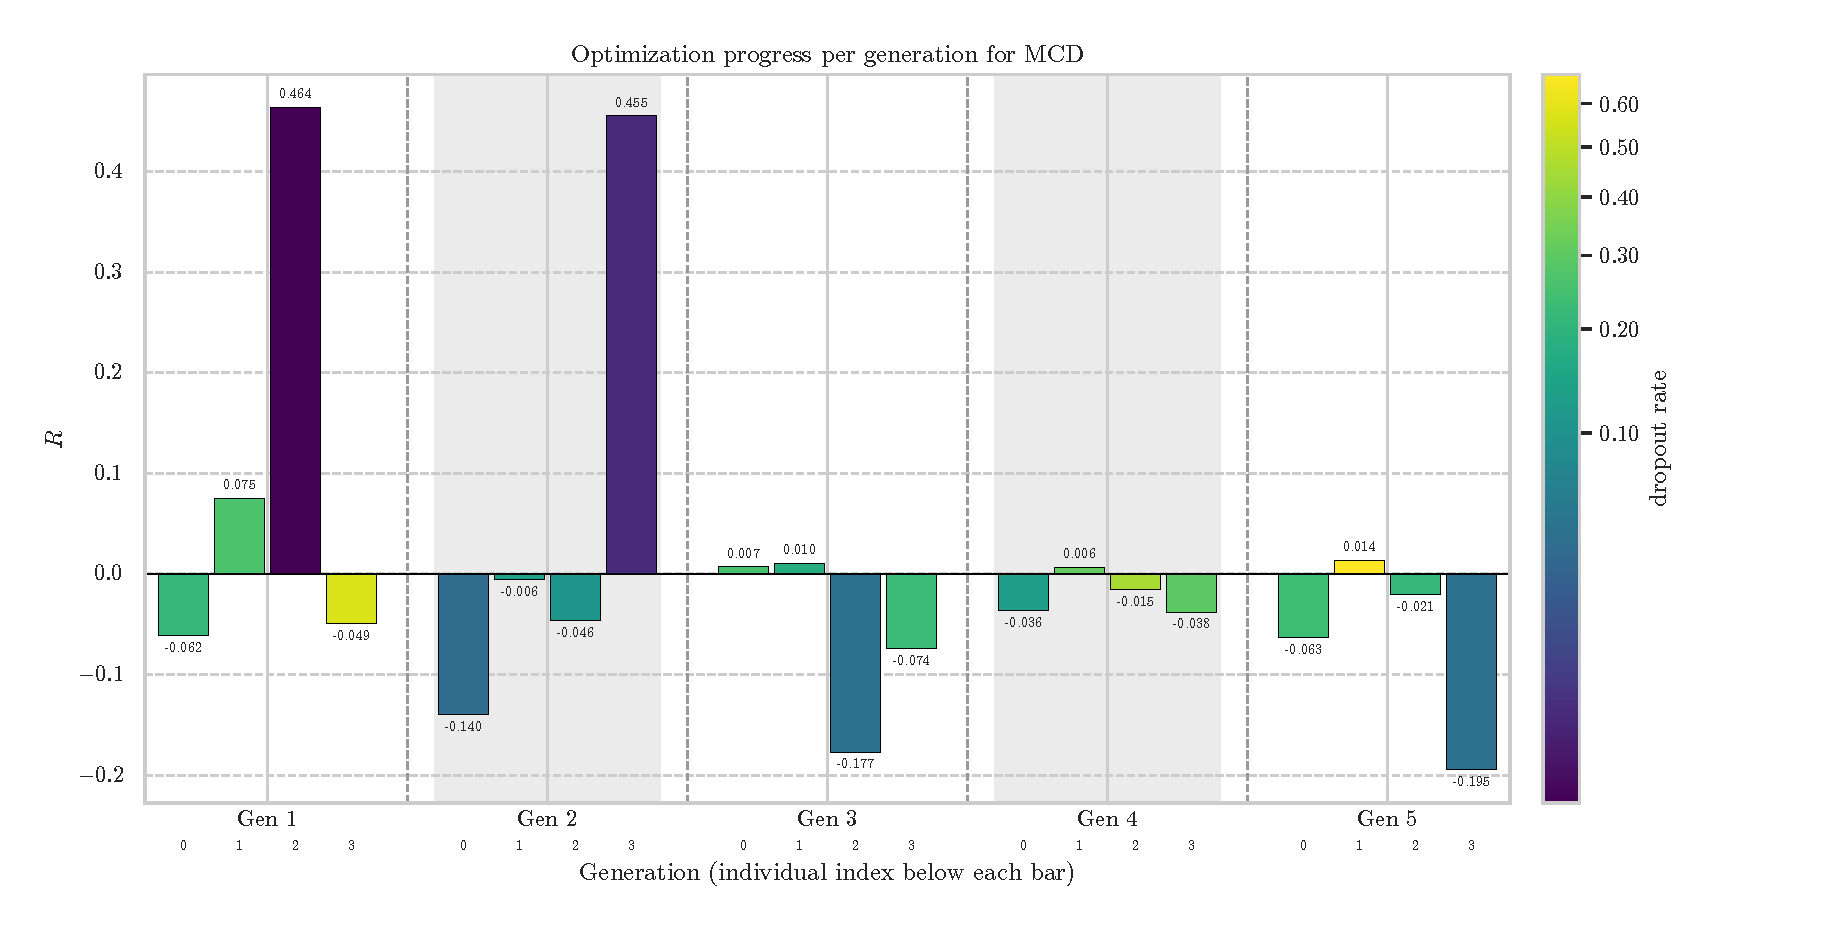
\includegraphics[width=0.9\linewidth]{../images/mcd_evolution_history.eps}
    \caption{Evolution history of the correlation coefficient ($R$) for the \acrshort{mcd} method.}
    \label{fig:mcd_evolution_history}
\end{figure}

The \acrshort{mcd} evolution in Figure \ref{fig:mcd_evolution_history} shows that the method is quite sensitive to hyperparameter tuning; the best performance on the calibration dataset is achieved with dropout rates $< 0.01$, beyond which performance drops sharply and the variance across the population increases dramatically. This suggests an unstable optimization landscape and a very narrow optimal range, which can be a problem for tuning this method in practice. The best performance is achieved with a dropout rate of $\mcdRate$ and a mean $R$ of $\mcdCalibrationR$ across folds. This rate is much lower than the commonly used $0.1$ or $0.2$ and is consistent with the findings of \cite{rodriguez2024uncertainty}.

\begin{figure}[htbp]
    \centering
    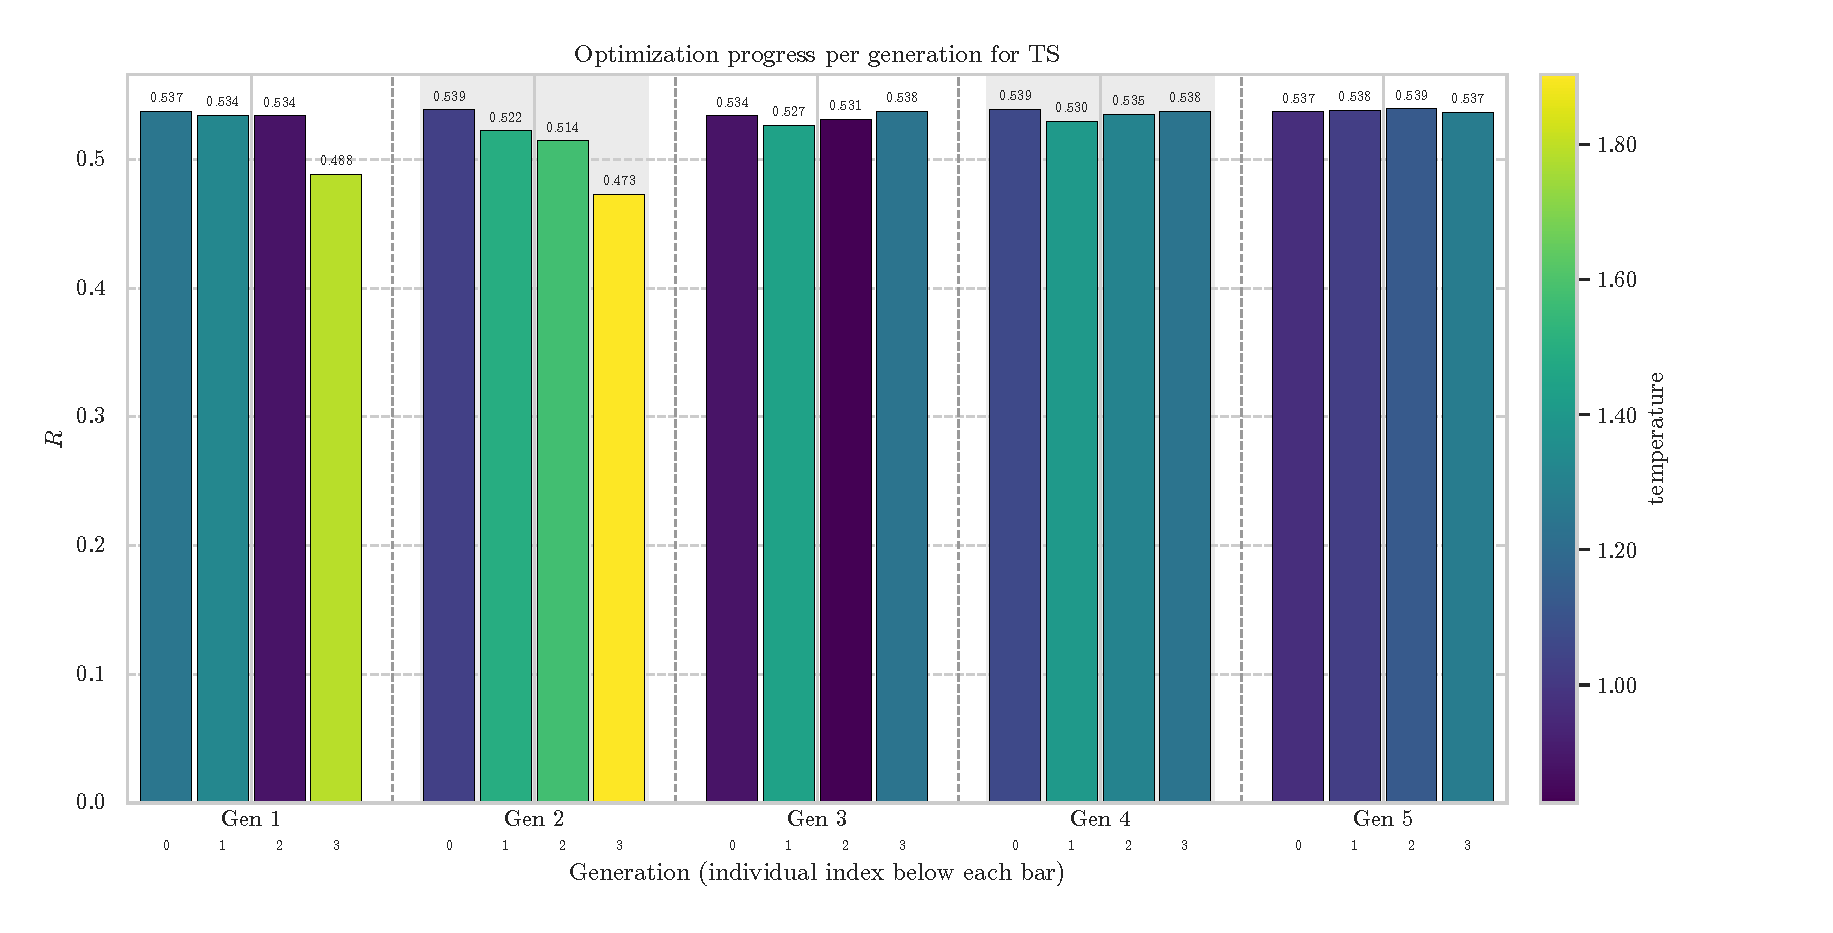
\includegraphics[width=0.9\linewidth]{../images/ts_evolution_history.eps}
    \caption{Evolution history of the correlation coefficient ($R$) for the \acrshort{ts} method.}
    \label{fig:ts_evolution_history}
\end{figure}

In contrast, Figure \ref{fig:ts_evolution_history} shows that \acrshort{ts} provides consistent uncertainty estimates across a wide range of temperature values, with the best performance achieved around $\tau = \tsTemp$ and a mean $R$ of $\tsCalibrationR$ across folds. Even at the sampled extremes, performance varies less than for the dropout-based methods, suggesting that \acrshort{ts} is less sensitive to hyperparameter selection in this experiment and may be a practical choice when computational resources for tuning are limited.

\begin{figure}[htbp]
    \centering
    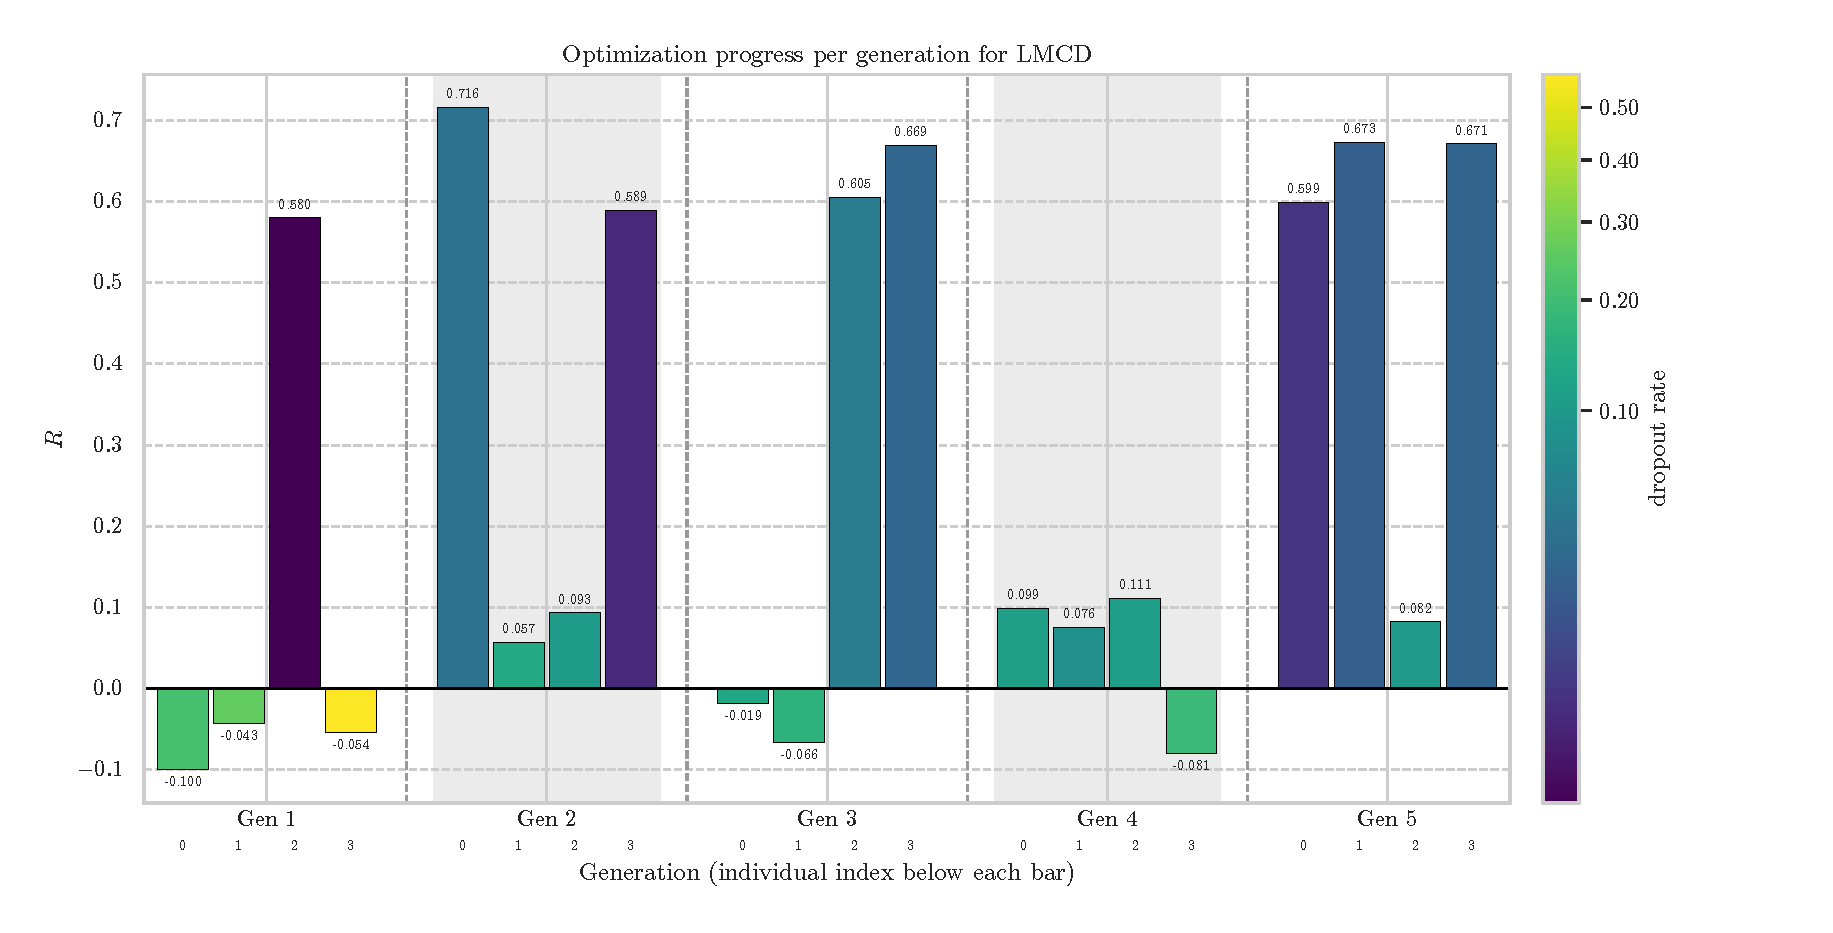
\includegraphics[width=0.9\linewidth]{../images/lmcd_evolution_history.eps}
    \caption{Evolution history of the correlation coefficient ($R$) for the \acrshort{lmcd} method.}
    \label{fig:lmcd_evolution_history}
\end{figure}

Figure \ref{fig:lmcd_evolution_history} shows that \acrshort{lmcd} follows a pattern similar to \acrshort{mcd}, where lower dropout ranges provide the best performance, but it remains more stable across a wider range of values. The best performance is achieved with a dropout rate of $\lmcdRate$ and a mean $R$ of $\lmcdCalibrationR$ across folds. \acrshort{lmcd} thus supports the trend of lower dropout rates yielding better performance, although its optimum is an order of magnitude higher than that of \acrshort{mcd}, which indicates that \acrshort{lmcd} is more robust to changes in the dropout rate and therefore easier and cheaper to tune.

\begin{figure}[htbp]
    \centering
    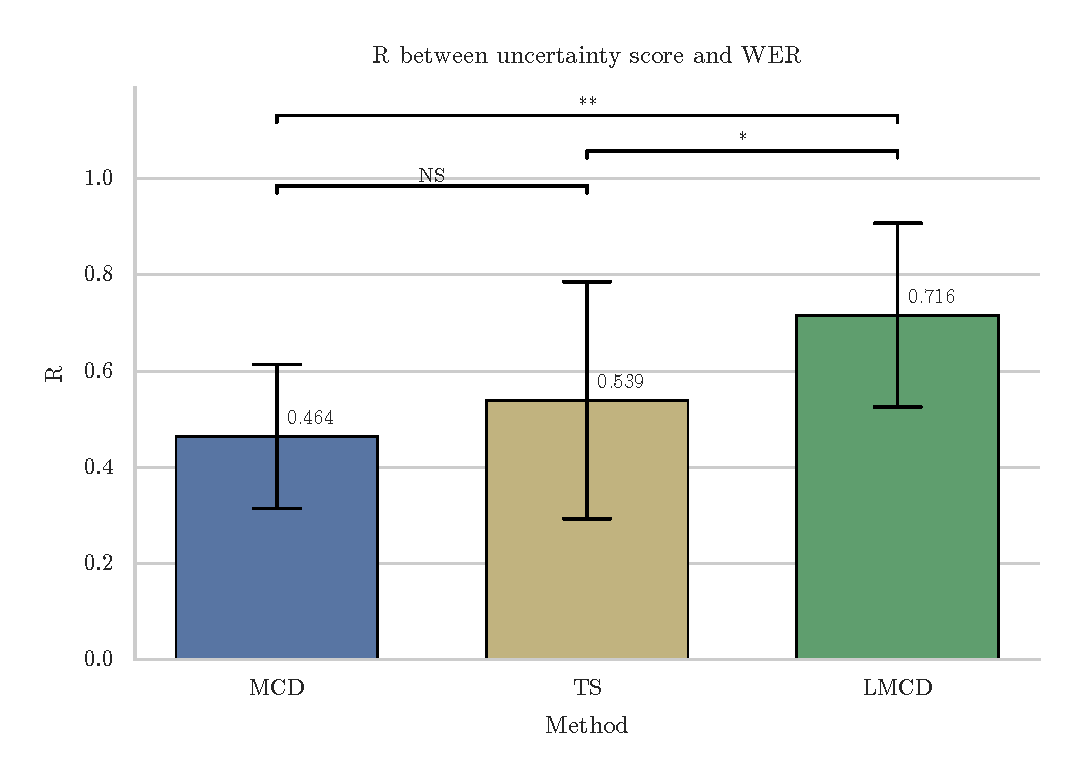
\includegraphics[width=0.9\linewidth]{../images/best_calibration.eps}
    \caption{Best calibration results for each \acrshort{uq} method. The whiskers represent the standard deviation of the $R$ values across folds.}
    \label{fig:best_calibration_results}
\end{figure}

Figure \ref{fig:best_calibration_results} summarizes the best calibration results for each method.

\subsection{Test Results}

Having selected the best hyperparameters on the calibration split, we evaluate them on the held-out test split. Figure \ref{fig:best_test_results} summarizes the best test results for each method, and the per-method values are collected in Table \ref{tab:summary}.

\begin{figure}[htbp]
    \centering
    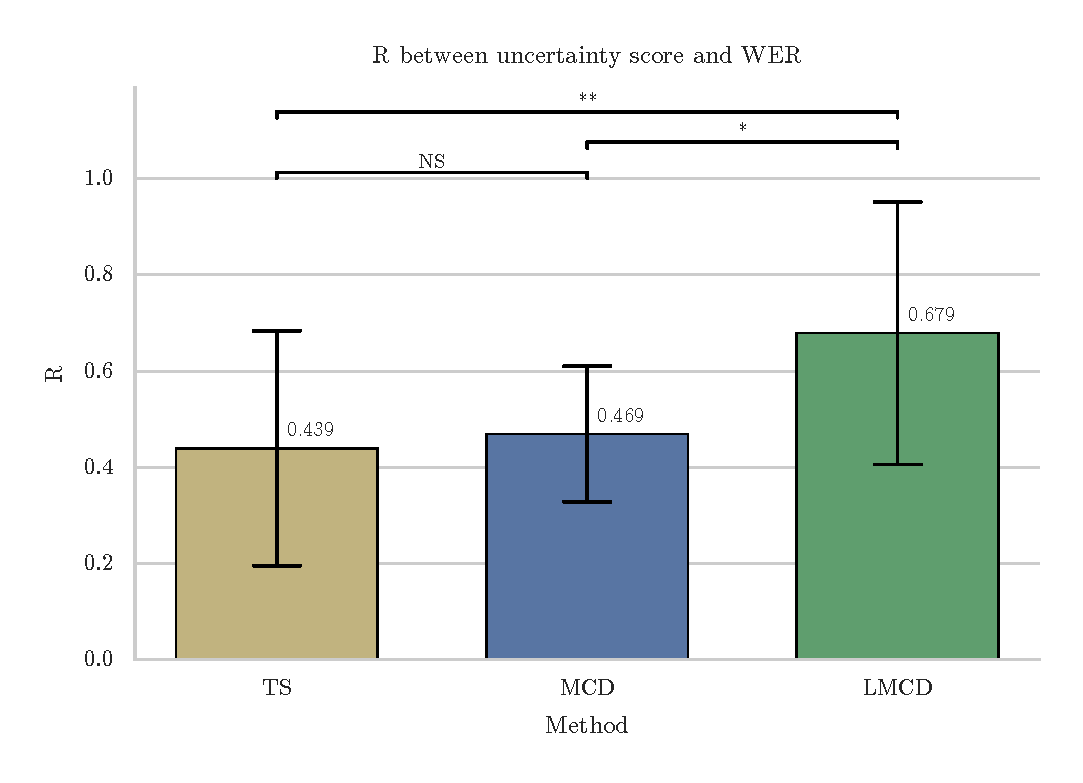
\includegraphics[width=0.9\linewidth]{../images/best_test.eps}
    \caption{Best test results for each \acrshort{uq} method. The whiskers represent the standard deviation of the $R$ values across folds.}
    \label{fig:best_test_results}
\end{figure}

\section{Statistical Tool Assumptions Tests}
\todo{aplicar normalidad y homocedasticidad tests a los $R$ values para justificar el uso de un t-test, o decidir usar un test no paramétrico.}

The statistical tool used is the Wilcoxon signed-rank test, a non-parametric test that operates on the ranks of the paired differences and therefore does not assume that the $R$ values are normally distributed. Because no normality or homoscedasticity assumption is required, there are no distributional assumptions to verify before applying it; the only requirements are that the observations be paired across folds and measured on at least an ordinal scale, both of which hold by construction since every method is evaluated on the same ten folds.

\section{Statistical Tool Results}

\subsection{Validity}

Table \ref{tab:wilcoxon_single_calibration} reports a one-sided Wilcoxon signed-rank test of whether each method's median $R$ is greater than zero across the ten folds, at $\alpha = 0.05$. All three methods reject the null hypothesis at $p = 0.0009766$, the smallest value attainable with $N = 10$, which corresponds to every fold yielding a positive correlation. This establishes that each method produces uncertainty scores that are consistently and positively correlated with the \acrshort{wer}, but it does not by itself rank the methods.

\begin{table}[ht]
    \centering
    \begin{tabular}{|l|l|l|l|l|}
        \hline
        Method          & N  & Median & p-value   & Verdict     \\ \hline
        \acrshort{mcd}  & 10 & 0.5068 & 0.0009766 & Significant \\ \hline
        \acrshort{ts}   & 10 & 0.6634 & 0.0009766 & Significant \\ \hline
        \acrshort{lmcd} & 10 & 0.7965 & 0.0009766 & Significant \\ \hline
    \end{tabular}
    \caption{Wilcoxon signed-rank validity test on the calibration dataset.}
    \label{tab:wilcoxon_single_calibration}
\end{table}

Table \ref{tab:wilcoxon_single_test} repeats the one-sided validity evaluation on the held-out test split. The null hypothesis is again rejected for every method ($p \leq 0.001953$), confirming that the positive correlation between uncertainty and \acrshort{wer} persists on data that was not used for hyperparameter selection.

\begin{table}[ht]
    \centering
    \begin{tabular}{|l|l|l|l|l|}
        \hline
        Method          & N  & Median & p-value   & Verdict     \\ \hline
        \acrshort{mcd}  & 10 & 0.4658 & 0.0009766 & Significant \\ \hline
        \acrshort{ts}   & 10 & 0.4262 & 0.001953  & Significant \\ \hline
        \acrshort{lmcd} & 10 & 0.7888 & 0.001953  & Significant \\ \hline
    \end{tabular}
    \caption{Wilcoxon signed-rank validity test on the test dataset.}
    \label{tab:wilcoxon_single_test}
\end{table}

\subsection{Pairwise Comparison}

Given that the validity test holds on both splits, we compare the methods with a paired, two-sided Wilcoxon signed-rank test at $\alpha = 0.05$. Table \ref{tab:wilcoxon_pairwise} reports the pairwise p-values on both splits. On the calibration split, \acrshort{lmcd} differs significantly from both \acrshort{mcd} ($p = 0.0020$) and \acrshort{ts} ($p = 0.027$), whereas \acrshort{mcd} and \acrshort{ts} are statistically indistinguishable ($p = 0.084$). The same ranking carries over to the held-out test split, where \acrshort{lmcd} remains significantly distinct from both \acrshort{mcd} ($p = 0.020$) and \acrshort{ts} ($p = 0.0059$), while \acrshort{mcd} and \acrshort{ts} stay indistinguishable ($p = 0.49$).

\begin{table}[ht]
    \centering
    \begin{tabular}{|l|l|l|}
        \hline
        Comparison                        & Calibration p-value & Test p-value \\ \hline
        \acrshort{lmcd} vs \acrshort{mcd} & 0.0020              & 0.020        \\ \hline
        \acrshort{lmcd} vs \acrshort{ts}  & 0.027               & 0.0059       \\ \hline
        \acrshort{mcd} vs \acrshort{ts}   & 0.084               & 0.49         \\ \hline
    \end{tabular}
    \caption{Pairwise two-sided Wilcoxon signed-rank test p-values between methods on the calibration and test datasets.}
    \label{tab:wilcoxon_pairwise}
\end{table}

\section{Obtained Metrics}

Table \ref{tab:summary} collects the optimal hyperparameter and the mean Pearson correlation between the uncertainty score and the \acrshort{wer}, averaged across the ten folds, for each method on both splits. \acrshort{lmcd} attains the highest correlation on the test split ($\lmcdTestR$), ahead of \acrshort{mcd} ($\mcdTestR$) and \acrshort{ts} ($\tsTestR$), and stays close to its calibration value, whereas \acrshort{ts} degrades the most between calibration and test.

\begin{table}[ht]
    \centering
    \begin{tabular}{|l|c|c|c|}
        \hline
        Method          & Optimal hyperparameter & Calibration $R$   & Test $R$   \\ \hline
        \acrshort{ts}   & $\tau = \tsTemp$       & \tsCalibrationR   & \tsTestR   \\ \hline
        \acrshort{mcd}  & dropout $= \mcdRate$   & \mcdCalibrationR  & \mcdTestR  \\ \hline
        \acrshort{lmcd} & dropout $= \lmcdRate$  & \lmcdCalibrationR & \lmcdTestR \\ \hline
    \end{tabular}
    \caption{Optimal hyperparameter and mean Pearson correlation ($R$) between the uncertainty score and \acrshort{wer}, averaged across the ten folds, for each \acrshort{uq} method on the calibration and test splits.}
    \label{tab:summary}
\end{table}

Throughout this chapter each method is summarized by its mean $R$ across folds, whereas the validity tables report the median $R$ on which the Wilcoxon test operates; the mean falls below the median for every method because one fold consistently yields a markedly lower, and for some methods slightly negative, correlation that pulls the average down.
\newpage

%Disussion

\chapter{Discussion}
\epigraph{``Another quote.''}{\vspace{10pt}Another Author}
\label{chapter:discussion}

\newpage

This chapter presents the analysis and discussion of the results shown in chapter \nameref{chapter:results}.

\section{Interpretation of the Results}

The clearest outcome is that \acrshort{lmcd} produces uncertainty scores that track the \acrshort{wer} substantially better than the two baselines, and that it is the only method separated from the others by a statistically significant margin on both splits. Its advantage over \acrshort{ts} is significant but more modest than its advantage over \acrshort{mcd}, which indicates that the distance-based estimation of \acrshort{lmcd} outperforms both the variance-based estimation of \acrshort{mcd} and the post-hoc calibration of \acrshort{ts}. The fact that \acrshort{mcd} and \acrshort{ts} remain statistically indistinguishable on both splits reinforces that the gain comes specifically from summarizing the disagreement among sampled transcriptions as an edit distance, rather than from sampling alone.

A second observation is the role of hyperparameter tuning. Both dropout-based methods only become informative at dropout rates well below the usual $0.1$--$0.2$ defaults, and \acrshort{mcd} in particular has a narrow region of useful values, outside of which its correlation collapses and its variance across folds grows. \acrshort{lmcd} shares the preference for low dropout but tolerates a wider range, which makes it easier and cheaper to tune. Without a tuning procedure applied on equal footing, this behavior would be easy to miss, and a poorly chosen default would have made the dropout-based methods look far weaker than they are.

A third observation concerns robustness to distribution shift. \acrshort{lmcd} and \acrshort{mcd} keep almost the same correlation when moving from calibration to test data, whereas \acrshort{ts} degrades the most. This is consistent with prior reports that the temperature is tied to the distribution of the calibration data and is therefore sensitive to data shift \cite{yu2022robust}\cite{mozafari2018attended}. In a deployment where the calibration set is not fully representative of the data the model will see, this fragility makes \acrshort{ts} a riskier choice than its low tuning cost might suggest.

\section{Practical Implications}

An uncertainty score that correlates with the \acrshort{wer} at $R \approx \lmcdTestR$ is directly useful: it can flag likely-erroneous transcriptions for human review, or drive a selective-transcription workflow in which only low-confidence utterances are escalated. \acrshort{lmcd} is the most capable of the three methods for this purpose and, like \acrshort{mcd}, it remains stable under distribution shift. The additional inference cost of a dropout-based method, which performs several stochastic passes per audio, is the price for that reliability and is justified when accurate uncertainty matters or the compute budget allows.

\section{On the Hypothesis}

The hypothesis set an aspirational target of a Pearson coefficient of $0.9$. The strongest method evaluated, \acrshort{lmcd}, reaches a mean $R$ of $\lmcdTestR$ (median $0.789$) on the held-out test split, so the absolute target of $0.9$ was not reached. The main objective, however, was framed as improving on the baseline of \cite{rodriguez2024uncertainty} by at least \qty{20}{\percent} in correlation with the \acrshort{wer}, and this was achieved: \acrshort{lmcd} raises the \acrshort{mcd} baseline from $\mcdTestR$ to $\lmcdTestR$, a relative gain of roughly \qty{45}{\percent}. The remaining gap to $0.9$ indicates that, while distance-based scoring is clearly the most informative of the three methods, there is still room for a dedicated method to close the distance, which is left as future work.

\section{Methodological Caveat}

The three methods do not all evaluate the \acrshort{wer} on the same transcription. \acrshort{ts} and \acrshort{mcd} report the \acrshort{wer} of a clean, dropout-free decoding, while \acrshort{lmcd} reports the \acrshort{wer} of the stochastic medoid it selects. This is faithful to each method's definition, but it means the mean \acrshort{wer} differs slightly across methods, so the comparison should be read as a comparison of uncertainty quality given each method's own predicted transcription, rather than over an identical set of transcriptions.

\section{Limitations}

Several limitations bound the scope of these conclusions. First, the SpaTrans \acrshort{uq} Bench comprises roughly 66 minutes of speech across 600 short utterances; while this is enough to expose clear and statistically consistent differences between methods, the absolute $R$ values and optimal hyperparameters may not transfer directly to larger corpora or other domains. Second, the optimization budget was deliberately small, a population of $4$ over $5$ generations, i.e.\ $20$ evaluations per method, dictated by the cost of repeated stochastic inference; a larger budget could refine the optima, particularly for \acrshort{mcd}, whose narrow region of useful dropout values makes it sensitive to under-sampling. Third, each method exposes a single scalar hyperparameter, so the use of \acrshort{cmaes} exercises only a one-dimensional slice of its capabilities, and it was not benchmarked against other tuners such as random \cite{bergstra2012random} or Bayesian \cite{snoek2012practical} search, leaving the most economical optimizer an open question. Fourth, the evaluation relies on the Pearson correlation, which captures linear association; a strongly monotonic but non-linear relationship between uncertainty and \acrshort{wer} could be understated. Finally, all experiments use a single model, Whisper base, and a single language, Spanish, so generalization to other architectures, model sizes, and languages remains to be verified.



%Conclusions and future work
\chapter{Conclusions and Future Work}
\epigraph{``Another quote.''}{\vspace{10pt}Another author}
\label{chapter:conclusions-fw}

\newpage

This chapter presents the final conclusions obtained through the research effort and the future work that can be derived.

\section{Conclusions}

\begin{itemize}

    \item Three sequence-level \acrshort{uq} methods for Spanish \acrshort{asr}, \acrshort{ts}, \acrshort{mcd}, and \acrshort{lmcd}, were tuned under a common \acrshort{cmaes} protocol and compared. \acrshort{lmcd} produces uncertainty scores that track the \acrshort{wer} substantially better than the two baselines and is the only method separated from them by a statistically significant margin on both the calibration and the test splits.

    \item Tuning on equal footing was instrumental in reaching this conclusion. The dropout-based methods only become informative at dropout rates far below the usual $0.1$--$0.2$ defaults, which underscores how sensitive the quality of an uncertainty estimate is to a single hyperparameter and how misleading an untuned comparison would have been.

    \item \acrshort{lmcd} and \acrshort{mcd} remain stable when moving from calibration to test data, whereas \acrshort{ts} degrades the most; the temperature is tied to the calibration distribution and is therefore the most fragile under distribution shift.

    \item At a correlation of $R \approx \lmcdTestR$ with the \acrshort{wer}, the \acrshort{lmcd} score is practically useful for flagging likely-erroneous transcriptions for human review or for driving selective transcription, at the cost of the extra inference required by the stochastic passes.

    \item The aspirational target of a Pearson coefficient of $0.9$ was not reached, but the main objective of improving on the baseline of \cite{rodriguez2024uncertainty} by at least \qty{20}{\percent} was met, with \acrshort{lmcd} improving the \acrshort{mcd} baseline by roughly \qty{45}{\percent} on the test split.

\end{itemize}


\section{Future Work}

\begin{itemize}
    \item Validate these findings on larger corpora, additional languages, and larger Whisper variants, to confirm that the ranking and the very low optimal dropout rates generalize beyond the current setting.

    \item Explore cheaper tuning strategies for the dropout-based methods and benchmark \acrshort{cmaes} against other tuners such as random \cite{bergstra2012random} and Bayesian \cite{snoek2012practical} search.

    \item Align the reported transcription across methods so that the \acrshort{wer} is computed on the same prediction for every method, strengthening direct comparison.

    \item Extend the evaluation to other agreement-based tasks, such as machine translation and open-ended generation, where the same distance-based scoring may apply.

    \item \todo{Future thread: propose a dedicated novel clear-box method to close the remaining gap to $0.9$, propose one or more reliability metrics beyond Pearson correlation, and evaluate \acrfull{fde} alongside the current methods.}
\end{itemize}

%Appendix

\chapter{Appendixes}
\label{chapter:appendixes}

\newpage

\section{Source Code}

\label{deliverable:source-code}

The full implementation of the test-bench, including the three \acrshort{uq} methods, the \acrshort{cmaes} optimization loop, and the evaluation pipeline, is available in the project repository.\todo{Add the public Git repository URL.} The per-fold fine-tuned Whisper models are published on the Hugging Face Hub as \texttt{danrdz/whisper-finetuned-es-modelo\_01} through \texttt{\_10}, and the dataset is published as \texttt{saul1917/SpaTrans\_UQ\_Bench\_raw}.

\section{Gathered Data from the Experiments}

Table \ref{tab:per_fold_r} reports the per-fold Pearson correlation $R$ between each method's uncertainty score and the \acrshort{wer} on the held-out test split, from which the mean values in Table \ref{tab:summary} are computed. Fold $10$ yields a markedly lower, and for \acrshort{ts} and \acrshort{lmcd} slightly negative, correlation for every method; this is the fold that pulls the mean below the median, as discussed in the \nameref{chapter:results} chapter.

\begin{table}[ht]
    \centering
    \begin{tabular}{|c|c|c|c|}
        \hline
        Fold & \acrshort{ts} $R$ & \acrshort{mcd} $R$ & \acrshort{lmcd} $R$ \\ \hline
        1    & 0.6636            & 0.6480             & 0.8040              \\ \hline
        2    & 0.3952            & 0.4467             & 0.7832              \\ \hline
        3    & 0.4485            & 0.5463             & 0.7943              \\ \hline
        4    & 0.6559            & 0.3894             & 0.5712              \\ \hline
        5    & 0.6750            & 0.6509             & 0.8303              \\ \hline
        6    & 0.2272            & 0.3564             & 0.6989              \\ \hline
        7    & 0.4039            & 0.4180             & 0.7973              \\ \hline
        8    & 0.3272            & 0.4848             & 0.7449              \\ \hline
        9    & 0.6753            & 0.5598             & 0.8306              \\ \hline
        10   & -0.0785           & 0.1899             & -0.0664             \\ \hline
        Mean & \tsTestR          & \mcdTestR          & \lmcdTestR          \\ \hline
    \end{tabular}
    \caption{Per-fold Pearson correlation $R$ between the uncertainty score and the \acrshort{wer} on the held-out test split, for each \acrshort{uq} method.}
    \label{tab:per_fold_r}
\end{table}




% Final pages
\backmatter

% Use single space
\singlespacing

% Acronyms
\clearpage
\chapter{Glossaries}
\printnoidxglossary[type=\acronymtype]


% Bibliography
\cleardoublepage
\renewcommand{\bibname}{References}

\refstepcounter{chapter}
\addcontentsline{toc}{chapter}{\bibname}
\bibliographystyle{plainnat}
\bibliography{references}{}

\doublespacing



\end{document}
